\section{ỨNG DỤNG HÌNH HỌC CỦA TÍCH PHÂN}
\subsection{Diện tích hình thang cong}
\subsubsection{Hình phẳng giới hạn bởi đồ thị hàm số, trục hoành và hai đường thẳng $x=a$ và $x=b$}
\begin{center}
	\begin{tikzpicture}[scale=1,font=\footnotesize,line join=round,line cap=round,>=stealth]
	% Draw axes
	\draw[->] (-0.5,0) -- (6,0) node[right] {$x$};
	\draw[->] (0,-0.5) -- (0,4) node[above] {$y$};
	
	% Labels
	\node at (0,0) [below left] {$O$};
	\node at (0.7,0) [below] {$a$};
	\node at (4.3,0) [below] {$b$};
	\node at (5.3,2) {$y = f(x)$};
	
	% Draw function curve
	\draw[thick,domain=0.5:4.7,samples=100] plot (\x,{-0.3*(\x-0.8)*(\x-2.5)*(\x-5)+1.5});
	
	% Draw vertical lines
	\draw[dashed] (0.7,0) -- (0.7,{-0.3*(0.7-0.8)*(0.7-2.5)*(0.7-5)+1.5});
	\draw[dashed] (4.3,0) -- (4.3,{-0.3*(4.3-0.8)*(4.3-2.5)*(4.3-5)+1.5});
	
	% Draw shaded area
	\fill[pattern=north east lines, pattern color=black!50] 
	(0.7,0) -- plot[domain=0.7:4.3,samples=100] (\x,{-0.3*(\x-0.8)*(\x-2.5)*(\x-5)+1.5}) -- (4.3,0) -- cycle;
	
	% Additional labels
	\node at (0.5,2.7) [below] {$x = a$};
	\node at (4.5,3.5) [below] {$x = b$};
	\node at (3.5,-0.1) [below left] {$y = 0$};
\end{tikzpicture}
\end{center}
Cho hàm số $y=f(x)$ liên tục trên $[a;b]$. Khi đó, diện tích hình phẳng giới hạn bởi đồ thị hàm số $y=f(x)$, trục hoành $Ox$ $(y=0)$ và hai đường thẳng $x=a$ và $x=b$ được tính bởi công thức

	$$S=\displaystyle\int\limits_a^b \left|f(x)\right|\mathrm{\,d}x$$

\textbf{Chú ý:} Giả sử hàm số $y=f(x)$ liên tục trên $[a;b]$. Nếu $f(x)$ không đổi dấu trên $[a;b]$ thì

	$$\displaystyle\int\limits_a^b \left|f(x)\right|\mathrm{\,d}x=\displaystyle\left|\int\limits_a^b f(x)\mathrm{\,d}x\right|.$$

\subsubsection{Hình phẳng giới hạn bởi hai đồ thị hàm số và hai đường thẳng $x=a$ và $x=b$}

\begin{center}
	\begin{tikzpicture}[scale=1,font=\footnotesize,line join=round,line cap=round,>=stealth]
	% Draw axes
\draw[->] (-0.5,0) -- (6,0) node[right] {$x$};
\draw[->] (0,-0.5) -- (0,4) node[above] {$y$};

% Labels
\node at (0,0) [below left] {$O$};
\node at (0.7,0) [below] {$a$};
\node at (4.3,0) [below] {$b$};
\node at (5,3.1) {$y = f(x)$};
\node at (5,2.1) {$y = g(x)$};
% Draw function curve
\draw[thick,domain=1:3.7,samples=100] plot (\x,{sqrt(4-(\x-2.5)^2)+1.5});
\draw[thick,domain=0.9:3.9,samples=100] plot (\x,{-sqrt(4-(\x-2.5)^2)+3.3});

% Draw vertical lines
\draw[dashed] (1.2,0) -- (1.2,{sqrt(4-(1.2-2.5)^2)+1.5});
\draw[dashed] (3.4,0) -- (3.4,{sqrt(4-(3.4-2.5)^2)+1.5});

% Draw shaded area
\fill[pattern=north east lines, pattern color=black!50] 
(1.2,1.78) -- plot[domain=1.2:3.4,samples=100] (\x,{sqrt(4-(\x -2.5)^2)+1.5}) -- (3.4,1.514) -- plot[domain=1.2:3.4,samples=100] (\x,{-sqrt(4-(\x-2.5)^2)+3.3}) -- cycle;

% Additional labels
\node at (1.2,4) [below] {$x = a$};
\node at (3.4,4) [below] {$x = b$};

\end{tikzpicture}
\end{center}
Cho 2 hàm số $y=f(x)$ và $y=g(x)$ liên tục trên $[a;b]$. Khi đó diện tích của hình phẳng giới hạn bởi đồ thị hai hàm số $y=f(x)$ và $y=g(x)$ và hai đường thẳng $x=a$ và $x=b$ được tính bởi công thức
$$
S=\displaystyle\int_a^b|f(x)-g(x)|\mathrm{\,d}x
$$
\subsection{Thể tích hình khối}
\subsubsection{Thể tích của vật thể}
\begin{center}
\begin{tikzpicture}[scale=1,font=\footnotesize,line join=round,line cap=round,>=stealth]
	\draw plot[smooth,tension=.65] coordinates{(1,2) (2.5,2.3) (3.5,2.2)};
	\draw[dashed] plot[smooth,tension=.65] coordinates{(3.5,2.2) (4,2)};
	\draw plot[smooth,tension=.65] coordinates{(4,2) (5,2.2) (5.5,2.1)};
	\draw[dashed] plot[smooth,tension=.65] coordinates{(5.5,2.1) (6,2)};
	\draw plot[smooth,tension=.65] coordinates{(1,1) (2.3,0.5) (3.5,0.8)};
	\draw[dashed] plot[smooth,tension=.65] coordinates{(3.5,0.8) (4,1)};
	\draw plot[smooth,tension=.65] coordinates{(4,1) (5,0.7) (5.5,0.8)};
	\draw[dashed] plot[smooth,tension=.65] coordinates{(5.5,0.8) (6,1)};
	\draw[dashed] (1,1) arc (-90:90:.2 and 0.5);
	\draw (1,2) arc (90:270:.2 and 0.5);
	\draw[dashed] (4,1) arc (-90:90:.2 and 0.5);
	\draw (4,2) arc (90:270:.2 and 0.5);
	\draw (6,1) arc (-90:270:.2 and 0.5);
	\fill[pattern=north east lines] (4,1) arc (-90:90:.2 and 0.5)--(4,2) arc (90:270:.2 and 0.5)--cycle;
	\draw (-.5,0)--(0.5,0) (1,0)--(3.5,0) (4,0)--(5.5,0);
	\draw[dashed] (0.5,0)--(1,0) (3.5,0)--(4,0) (5.5,0)--(6,0);
	\draw[->] (6,0)--(7,0)node[below]{$x$};
	\draw (0.5,-1)--(0.5,3)--(1.5,3.5)--(1.5,2.2) (1.5,.8)--(1.5,-0.5)--(0.5,-1);
	\draw[dashed](1.5,2.2)--(1.5,.8);
	\draw[dashed] (1,1)--(1,0)node[below]{$a$};
	\coordinate (A) at (0.5,3);
	\coordinate (B) at (1.5,3.5);
	\coordinate (C) at (1.5,2.2);
	%\tkzMarkAngle[size=.6](A,B,C);
	\draw pic[draw=black, angle eccentricity=1.6, angle radius=0.5cm]{angle=A--B--C};
	\draw (1.3,3.2) node {\footnotesize $P$};
	\draw (3.5,-1)--(3.5,3)--(4.5,3.5)--(4.5,2) (4.5,1)--(4.5,-0.5)--(3.5,-1);
	\draw[dashed](4.5,2)--(4.5,1);
	\draw[dashed] (4,1)--(4,0)node[below]{$x$};
	\coordinate (D) at (3.5,3);
	\coordinate (E) at (4.5,3.5);
	\coordinate (F) at (4.5,2);
	%	\tkzMarkAngle[size=.6](D,E,F);
	\draw pic[draw=black, angle eccentricity=1.6, angle radius=0.5cm]{angle=D--E--F};
	\draw (4.3,3.2) node {\footnotesize $R$};
	\draw (5.5,-1)--(5.5,3)--(6.5,3.5)--(6.5,-0.5)--(5.5,-1);
	\draw[dashed] (6,1)--(6,0)node[below]{$b$};
	\coordinate (G) at (5.5,3);
	\coordinate (H) at (6.5,3.5);
	\coordinate (K) at (6.5,-0.5);
	%	\tkzMarkAngle[size=.6](G,H,K);
	\draw pic[draw=black, angle eccentricity=1.6, angle radius=0.5cm]{angle=G--H--K};	\draw (6.3,3.2) node {\footnotesize $Q$};
	\draw (0,.3) node {$O$};
	\fill (0,0) circle(1pt);
	\draw[->] (4,1.5)--(4.7,1.7) node[right] {\scriptsize $S(x)$};
\end{tikzpicture}
\end{center}
Trong không gian, cho một vật thể nằm trong khoảng không gian giữa hai mặt phẳng $(P)$ và $(Q)$ cùng vuông góc với trục $Ox$ tại các điểm $a$ và $b$. Mặt phẳng vuông góc với trục $Ox$ tại điểm $x(a\leq x \leq b)$ cắt vật thể theo mặt cắt có diện tích $S(x)$. Khi đó, nếu $S(x)$ là hàm số liên tục trên $[a;b]$ thì thể tích của vật thể được tính bởi công thức
	$$V=\displaystyle\int\limits_a^b S(x)\mathrm{\,d}x$$
\subsubsection{Thể tích khối tròn xoay}
\begin{center}
	\begin{tikzpicture}[scale=1,font=\footnotesize,line join=round,line cap=round,>=stealth]
	 \draw[->] (-1,0) -- (6,0) node[right] {$x$};
	\draw[->] (0,-3) -- (0,3) node[above] {$y$};
	
	\draw[black, thick] plot[domain=0.5:5] (\x, {0.8*(0.4*(\x-1)-0.4)^2+1});
	\draw[black, thick, dashed] plot[domain=0.5:5] (\x, {-0.8*(0.4*(\x-1)-0.4)^2-1});
	
	\draw[black, thick,dashed, domain=4.54:5.54, samples=100] plot (\x, {sqrt(4.63 * (1 - 4 * (\x - 5.04)^2))});
	\draw[black, thick,dashed, domain=4.54:5.54, samples=100] plot (\x, {-sqrt(4.63 * (1 - 4 * (\x - 5.04)^2))});
	
	
	\draw[thick,dashed,domain=0.5:1.50 ,samples=100] plot (\x,{sqrt(0.5^2-(\x -1)^2)*1.5*1.5});
	\draw[thick,dashed,domain=0.5:1.50,samples=100] plot (\x,-{sqrt(0.5^2-(\x-1)^2)*1.5*1.5});
	
	\draw[thick,dashed,domain=2.55:3.551,samples=100] plot (\x,-{sqrt(1.274-5.09*(\x-3.05)^2)});
	\draw[thick,dashed,domain=2.55:3.551,samples=100] plot (\x,{sqrt(1.274-5.09*(\x-3.05)^2)});
	
	% Additional labels
	\node at (1,0) [below] {$a$};
	\node at (3,0) [below] {$x$};
	\node at (5,0) [below] {$b$};
	\node at (0,0) [below left] {$O$};
	\node at (3,2) [below] {$y=f(x)$};
	% Draw vertical lines
	\draw[thick] (1,0) -- (1,{0.8*(0.4*(1-1)-0.4)^2+1});
	\draw[thick] (3,0) -- (3,{0.8*(0.4*(3-1)-0.4)^2+1});
	\draw[thick] (5,0) -- (5,{0.8*(0.4*(5-1)-0.4)^2+1});
	
	%fill
	% Draw shaded area
	\fill[pattern=north east lines, pattern color=black!50] 
	(1,0) -- plot[domain=1:5,samples=100] (\x,{0.8*(0.4*(\x-1)-0.4)^2+1}) -- (5,0) -- cycle;
	
\end{tikzpicture}
\end{center}

Cho hàm số $y=f(x)$ liên tục, không âm trên $[a;b]$. Hình phẳng $(H)$ giới hạn bởi đồ thị hàm số $y=f(x)$, trục hoành $O x$ và hai đường thẳng $x=a$ và $x=b$ quay quanh trục $O x$ tạo thành một khối tròn xoay có thể tích bằng

	$$V=\displaystyle\pi\int\limits_a^b \left[f(x)\right]^2\mathrm{\,d}x$$

\chude{TÍNH DIỆN TÍCH GIỚI HẠN BỞI CÁC ĐƯỜNG CONG}
\setcounter{subsubsection}{0}
\subsubsection{Dạng 1}
$\heva{y&=f(x)\\y&=0\\x&=a\\x&=b} \Rightarrow S=\displaystyle\int\limits_a^b \left|f(x)\right|\mathrm{\,d}x$
\begin{center}
	\begin{tikzpicture}
% Draw axes
\draw[->] (-0.5,0) -- (6,0) node[right] {$x$};
\draw[->] (0,-0.5) -- (0,4) node[above] {$y$};

% Labels
\node at (0,0) [below left] {$O$};
\node at (0.7,0) [below] {$a$};
\node at (4.3,0) [below] {$b$};
\node at (5.3,2) {$y = f(x)$};

% Draw function curve
\draw[thick,domain=0.5:4.7,samples=100] plot (\x,{-0.3*(\x-0.8)*(\x-2.5)*(\x-5)+1.5});

% Draw vertical lines
\draw[dashed] (0.7,0) -- (0.7,{-0.3*(0.7-0.8)*(0.7-2.5)*(0.7-5)+1.5});
\draw[dashed] (4.3,0) -- (4.3,{-0.3*(4.3-0.8)*(4.3-2.5)*(4.3-5)+1.5});

% Draw shaded area
\fill[pattern=north east lines, pattern color=black!50] 
(0.7,0) -- plot[domain=0.7:4.3,samples=100] (\x,{-0.3*(\x-0.8)*(\x-2.5)*(\x-5)+1.5}) -- (4.3,0) -- cycle;

% Additional labels
\node at (0.5,2.7) [below] {$x = a$};
\node at (4.5,3.5) [below] {$x = b$};
\node at (3.5,-0.1) [below left] {$y = 0$};
\end{tikzpicture}
\end{center}
\subsubsection{Dạng 2}
$\heva{y&=f(x)\\y&=g(x)\\x&=a\\x&=b} \Rightarrow S=\displaystyle\int\limits_a^b \left|f(x)-g(x)\right|\mathrm{\,d}x$

\begin{center}
	\begin{tikzpicture}[scale=1,font=\footnotesize,line join=round,line cap=round,>=stealth]
	% Draw axes
\draw[->] (-0.5,0) -- (6,0) node[right] {$x$};
\draw[->] (0,-0.5) -- (0,4) node[above] {$y$};

% Labels
\node at (0,0) [below left] {$O$};
\node at (0.7,0) [below] {$a$};
\node at (4.3,0) [below] {$b$};
\node at (5,3.1) {$y = f(x)$};
\node at (5,2.1) {$y = g(x)$};
% Draw function curve
\draw[thick,domain=1:3.7,samples=100] plot (\x,{sqrt(4-(\x-2.5)^2)+1.5});
\draw[thick,domain=0.9:3.9,samples=100] plot (\x,{-sqrt(4-(\x-2.5)^2)+3.3});

% Draw vertical lines
\draw[dashed] (1.2,0) -- (1.2,{sqrt(4-(1.2-2.5)^2)+1.5});
\draw[dashed] (3.4,0) -- (3.4,{sqrt(4-(3.4-2.5)^2)+1.5});

% Draw shaded area
\fill[pattern=north east lines, pattern color=black!50] 
(1.2,1.78) -- plot[domain=1.2:3.4,samples=100] (\x,{sqrt(4-(\x -2.5)^2)+1.5}) -- (3.4,1.514) -- plot[domain=1.2:3.4,samples=100] (\x,{-sqrt(4-(\x-2.5)^2)+3.3}) -- cycle;

% Additional labels
\node at (1.2,4) [below] {$x = a$};
\node at (3.4,4) [below] {$x = b$};

\end{tikzpicture}
\end{center}
\textbf{Chú ý:}
\begin{itemize}
\item Nếu $f(x)$ không đổi dấu trên $[a;b]$ thì $\displaystyle\int\limits_a^b \left|f(x)\right|\mathrm{\,d}x=\left|\displaystyle\int\limits_a^b f(x)\mathrm{\,d}x\right|$.

\item Khi đó diện tích của hình phẳng giới hạn bởi đồ thị hai hàm số nằm dưới trục hoành thì mang giá trị âm, còn nằm trên trục hoành thì mang giá trị dương.
\end{itemize}

\begin{dang}
	{TÍNH DIỆN TÍCH GIỚI HẠN BỞI CÁC ĐƯỜNG CONG KHI BIẾT HÀM SỐ CÁC ĐƯỜNG CONG}\end{dang}
\TN
\Opensolutionfile{ans}[ans/ans2-C4B3CD1-D1]
\begin{ex}%[2D4N3-1]
	Cho hai hàm số $f(x)$ và $g(x)$ liên tục trên $[a;b]$. Diện tích hình phẳng giới hạn bởi đồ thị của các hàm số $y=f(x), y=g(x)$ và các đường thẳng $x=a, x=b$ bằng
\choice
{$\left|\displaystyle\int\limits_a^b \left[f(x)-g(x)\right]\mathrm{\,d}x\right|$}
{$\displaystyle\int\limits_a^b \left|f(x)+g(x)\right|\mathrm{\,d}x$}
{\True $\displaystyle\int\limits_a^b \left|f(x)-g(x)\right|\mathrm{\,d}x$}
{$\displaystyle\int\limits_a^b \left[f(x)-g(x)\right]\mathrm{\,d}x$}
\loigiai{
Theo lý thuyết thì diện tích hình phẳng được giới hạn bởi đồ thị của các đường\\ $y=f(x), y=g(x)$, $x=a, x=b$ 
\\Được tính theo công thức $S=\displaystyle\int\limits_a^b \left|f(x)-g(x)\right|\mathrm{\,d}x$.
}
\end{ex}
\begin{ex}%[2D4N3-1]
	Gọi $S$ là diện tích của hình phẳng giới hạn bởi các đường $y=3^x$, $y=0$, $x=0$, $x=2$. Mệnh đề nào dưới đây đúng?
\choice
{\True $\displaystyle\int\limits_0^2 3^x\mathrm{\,d}x$}
{$S=\pi\displaystyle\int\limits_0^2 3^{2x}\mathrm{\,d}x$}
{$S=\pi\displaystyle\int\limits_0^2 3^x\mathrm{\,d}x$}
{$S=\displaystyle\int\limits_0^2 3^{2x}\mathrm{\,d}x$}

\loigiai{
Diện tích hình phẳng đã cho được tính bởi công thức $S=\displaystyle\int\limits_0^2 3^x\mathrm{\,d}x$.
}
\end{ex}%[2D4N3-1]
\begin{ex}%[2D4N3-1]
	Diện tích hình phẳng giới hạn bởi đồ thị hàm số $y=(x-2)^2-1$, trục hoành và hai đường thẳng $x=1, x=2$ bằng
\choice
{\True $\dfrac{2}{3}$}
{$\dfrac{3}{2}$}
{$\dfrac{1}{3}$}
{$\dfrac{7}{3}$}
\loigiai{
Ta có $S=\displaystyle\int\limits_1^2 \left|(x-2)^2-1\right|\mathrm{\,d}x=\displaystyle\int\limits_1^2\left|x^2-4 x+3\right| \mathrm{d}x=\left|\displaystyle\int\limits_1^2\left(x^2-4 x+3\right) \mathrm{d}x\right|=\dfrac{2}{3}$.
}

\end{ex}
\begin{ex}%[2D4H3-1]
	Tính diện tích $S$ hình phẳng giới hạn bởi các đường $y=x^2+1$, $x=-1$, $x=2$ và trục hoành.
\choice
{\True $S=6$}
{$S=16$}
{$S=\dfrac{13}{6}$}
{$S=13$}
\loigiai{
Ta có $S=\displaystyle\int\limits_{-1}^2\left|x^2+1\right| \mathrm{d}x=\displaystyle\int\limits_{-1}^2\left(x^2+1\right) \mathrm{d}x=6$.
}
\end{ex}
\begin{ex}%[2D4H3-1]
	Gọi $S$ là diện tích hình phẳng giới hạn bởi các đường $y=x^2+5, y=6 x, x=0, x=1$. Tính $S$.
\choice
{$\dfrac{4}{3}$}
{\True $\dfrac{7}{3}$}
{$\dfrac{8}{3}$}
{$\dfrac{5}{3}$}
\loigiai{
Diện tích hình phẳng cần tìm $S=\displaystyle\int\limits_0^1\left|x^2-6 x+5\right| \mathrm{d}x=\dfrac{7}{3}$.
}
\end{ex}
\begin{ex}%[2D4V3-1]
	Diện tích hình phẳng giới hạn bởi đồ thị các hàm số $y=\ln x, y=1$ và hai đường thẳng $x=1, x=e$ bằng
\choice
{$e^2$}
{$e+2$}
{$2 e$}
{\True $e-2$}
\loigiai{
\begin{eqnarray*}
S&=&\displaystyle\int\limits_1^e|\ln x-1|\mathrm{d}x\\&=&\left|\displaystyle\int\limits_1^e(\ln x-1) \mathrm{d}x\right|\\&=&|x(\ln x-1)|_1^e-\displaystyle\int\limits_1^e \mathrm{d}x|\\&=&| 1-\left.x\right|_1 ^e|\\&=&| 1-(e-1)|=| 2-e \mid\\&=&e-2.
\end{eqnarray*}
}
\end{ex}
\begin{ex}%[2D4H3-1]
	Diện tích hình phẳng giới hạn bởi đồ thị của hàm số $y=4 x-x^2, y=2 x$ và hai đường thẳng $x=1, x=e$ bằng
\choice
{$4$}
{$\dfrac{20}{3}$}
{\True $\dfrac{4}{3}$}
{$\dfrac{16}{3}$}
\loigiai{
	Diện tích hình phẳng cần tìm là\[S=\displaystyle\int\limits_0^2\left|x^2-2 x\right| \mathrm{d}x=\displaystyle\int\limits_0^2\left(2 x-x^2\right) \mathrm{d}x=\left.\left(x^2-\dfrac{x^3}{3}\right)\right|_0 ^2=\dfrac{4}{3}.\]
}
\end{ex}
\begin{ex}%[2D4V3-1]
	Tính diện tích $S$ của hình phẳng giới hạn bởi các đường $y=x^2-2 x$, $y=0$, $x=-10$, $x=10$.
\choice
{$S=\dfrac{2000}{3}$}
{$S=2008$}
{$S=2000$}
{\True $S=\dfrac{2008}{3}$}
\loigiai{
Phương trình hoành độ giao điểm của hai đường $(C)\colon y=x^2-2 x$ và $(d)\colon y=0$ là
$$
x^2-2 x=0 \Leftrightarrow\hoac{
	x=0 \\
	x=2
}.
$$
Bảng xét dấu\\
\begin{center}
	\begin{tikzpicture}
	\tkzTabInit[nocadre=false,lgt=2.5,espcl=2.5,deltacl=0.6]
	{$x$ /0.6, VT/0.6}
	{$-\infty$, $0$, $2$, $+\infty$}
	\tkzTabLine{,+,,-,,+,}
\end{tikzpicture}
\end{center}
Diện tích cần tìm

\begin{eqnarray*}
	S&=&\displaystyle\int\limits_{-10}^{10}\left|x^2-2 x\right| \mathrm{d}x\\&=&\displaystyle\int\limits_{-10}^0\left(x^2-2 x\right) \mathrm{d}x-\displaystyle\int\limits_0^2\left(x^2-2 x\right) \mathrm{d}x+\displaystyle\int\limits_2^{10}\left(x^2-2 x\right) \mathrm{d}x 
	\\&=&\left.\left(\dfrac{x^3}{3}-x^2\right)\right|_{-10} ^0-\left.\left(\dfrac{x^3}{3}-x^2\right)\right|_0 ^2+\left.\left(\dfrac{x^3}{3}-x^2\right)\right|_2 ^{10}\\&=&\dfrac{1300}{3}+\dfrac{4}{3}+\dfrac{704}{3}\\&=&\dfrac{2008}{3} .
\end{eqnarray*}
}
\end{ex}
\Closesolutionfile{ans}
% \indapan{10}{ans/ans2-C4B3CD1-D1}
\TNTF
\Opensolutionfile{ans}[ans/ans2-C4B3CD1-D1-DS]
\begin{ex}%[2D4N3-1]
	Gọi $S$ là diện tích của hình phẳng giới hạn bời các đường $y=2^x$, $y=0$, $x=0$, $x=2$. Các mệnh đề sau đây đúng hay sai?
\choiceTF
{\True $S=\displaystyle\int\limits_0^2 2^x \mathrm{d}x$}
{\True $S=\dfrac{3}{\ln 2}$}
{$S=\pi \displaystyle\int\limits_0^2 2^x \mathrm{d}x$}
{$S=\dfrac{3 \pi}{\ln 2}$}
\loigiai{
\[
S=\displaystyle\int\limits_0^2\left|2^x\right| \mathrm{d}x=\displaystyle\int\limits_0^2 2^x \mathrm{d}x=\dfrac{2^2}{\ln 2}-\dfrac{2^0}{\ln 2}=\dfrac{3}{\ln 2}\left( \text {do } 2^x>0, \forall x \in[0;2]\right) .
\]
}
\end{ex}
\begin{ex}%[2D4N3-1]
	Gọi $S$ là diện tích hình phẳng giới hạn bởi các đường $y=\mathrm{e}^x, y=0, x=0, x=2$. Các mệnh đề sau đây đúng hay sai?
\choiceTF
{\True $S=\displaystyle\int\limits_0^2 \mathrm{e}^x \mathrm{d}x$}
{$S=e^2$}
{$S=\pi \displaystyle\int\limits_0^2 \mathrm{e}^x \mathrm{d}x$}
{$S=\left(e^2-1\right) \pi$}
\loigiai{
Diện tích hình phẳng giới hạn bời các đường $y=\mathrm{e}^x, y=0, x=0, x=2$ là
\[
S=\displaystyle\int\limits_0^2 e^x \mathrm{d}x=e^2-1.
\]
}
\end{ex}
\begin{ex}%[2D4V3-1]
	Các mệnh đề sau đây đúng hay sai
\choiceTF
{\True Diện tích hình phẳng giới hạn bởi đồ thị hàm số $y=x^2$, $y=2 x$, $x=0$, $x=1$ là $\dfrac{4}{3}$}
{\True Diện tích hình phẳng giới hạn bởi đồ thị hàm số $y=-x^2+2 x+1$, $y=2 x^2-4 x+1$, $x=0$, $x=2$ là $4$}
{\True Diện tích hình phẳng giới hạn bởi đồ thị hàm số $y=\dfrac{x-1}{x+1}$, trục hoành, $x=0$, $x=1$ là $2 \ln 2-1$}
{\True Diện tích hình phẳng giới hạn bởi đồ thị hàm số $y=-x^3+12 x$, $y=-x^2$, $x=-3$, $x=4$ là $\dfrac{937}{12}$}
\loigiai{
\begin{itemchoice}
\itemch Đúng.\\Diện tích hình phẳng giới hạn bời đồ thị hàm số $y=x^2$, $y=2 x$, $x=0$, $x=1$ là
\begin{eqnarray*}
S&=&\displaystyle\int\limits_0^1\left|x^2-x\right| \mathrm{d}x\\&=&\left|\displaystyle\int\limits_0^1\left(x^2-x\right) \mathrm{d}x\right|\\&=&\dfrac{4}{3}.
\end{eqnarray*}

\itemch Đúng.\\Diện tích hình phẳng giới hạn bởi đồ thị hàm số $y=-x^2+2x+1$, $y=2 x^2-4 x+1$, $x=0$, $x=2$ là
\begin{eqnarray*}
&&\displaystyle\int\limits_0^2\left|2x^2-4x+1-\left(-x^2+2 x+1\right)\right| \mathrm{d}x
\\&=&\displaystyle\int\limits_0^2\left|3 x^2-6 x\right| \mathrm{d}x
\\&=&\displaystyle\int\limits_0^2\left(6 x-3 x^2\right) \mathrm{d}x
\\&=&\left(3 x^2-x^3\right)|_0^2=4.
\end{eqnarray*}

\itemch Đúng.\\Diện tích hình phẳng giới hạn bởi đồ thị hàm số $y=\dfrac{x-1}{x+1}$, trục hoành, $x=0$, $x=1$ là

\begin{eqnarray*}
S&=&\displaystyle\int\limits_0^1\left|\dfrac{x-1}{x+1}\right| \mathrm{d}x
\\&=&\left|\displaystyle\int\limits_0^1\left(\dfrac{x-1}{x+1}\right)\mathrm{d}x\right|
\\&=&\left|\displaystyle\int\limits_0^1\left(1-\dfrac{2}{x+1}\right)\mathrm{d}x\right|
\\&=&|(x-2 \ln |x+1|)|_0^1|
\\&=&2 \ln {2}-1.
\end{eqnarray*}
\itemch Đúng.\\Diện tích hình phẳng giới hạn bởi đồ thị hàm số $y=-x^3+12$, $y=-x^2$, $x=-3$ là

\begin{eqnarray*}
	S&=&\displaystyle\int\limits_{-3}^4\left|x^3-x^2-12x\right| \mathrm{d}x
	\\&=&\displaystyle\int\limits_{-3}^0\left|x^3-x^2-12x\right| \mathrm{d}x+\displaystyle\int\limits_0^4\left|x^3-x^2-12 x\right| \mathrm{d}x 
	\\&=&\left|\displaystyle\int\limits_{-3}^0\left(x^3-x^2-12 x\right) \mathrm{d}x\right|+\left|\displaystyle\int\limits_0^4\left(x^3-x^2-12 x\right) \mathrm{d}x\right|
	\\&=&\left| \left|\left(\dfrac{x^4}{4}-\dfrac{x^3}{3}-6 x^2\right)\right|_{-3}^0\right| +\left| \left(\dfrac{x^4}{4}-\dfrac{x^3}{3}-6 x^2\right)\right|_0^4
	\\&=&\left|\dfrac{-99}{4}\right|+\left|\dfrac{-160}{3}\right|=\dfrac{937}{12}.
\end{eqnarray*}
\end{itemchoice}
}
\end{ex}
\Closesolutionfile{ans}
% \indapan{3}{ans/ans2-C4B3CD1-D1-DS}
\TN
\Opensolutionfile{ans}[ans/ans2-C4B3CD1-D1-KQ]
\begin{ex}%[2D4V3-1]
	Tính diện tích hình phẳng giới hạn bời đồ thị hàm số $y=x^2+x-1$, $y=x^4+x-1$, $x=-1$, $x=1$.
\shortans{$0,27$}
\loigiai{
Diện tích hình phẳng giới hạn bởi đồ thị hàm số $y=x^2+x-1, y=x^4+x-1, x=-1, x=1$ là
\begin{eqnarray*}
	S&=&\displaystyle\int\limits_{-1}^1\left|x^2-x^4\right| \mathrm{d}x\\
	&=&\displaystyle\int\limits_{-1}^0\left|x^2-x^4\right| \mathrm{d}x+\displaystyle\int\limits_0^1\left|x^2-x^4\right| \mathrm{d}x\\
	&=&\left|\displaystyle\int\limits_{-1}^0\left(x^2-x^4\right) \mathrm{d}x\right|+\left|\displaystyle\int\limits_0^1\left(x^2-x^4\right) \mathrm{d}x\right|\\
	&=&\left|\left(\dfrac{x^3}{3}-\dfrac{x^5}{5}\right)\right| 0|+|\left(\dfrac{x^3}{3}-\dfrac{x^5}{5}\right)|0|\\
	&=&\dfrac{2}{15}+\dfrac{2}{15}=\dfrac{4}{15}\approx0,27.
\end{eqnarray*}
}
\end{ex}

\begin{ex}%[2D4V3-1]
	Kí hiệu $S(t)$ là diện tích của hình phẳng giới hạn bởi các đường $y=2 x+1$, $y=0$, $x=1$, $x=t\left(t>1\right)$. Tìm $t$ để $S(t)=10$.
\shortans{$3$}
\loigiai{
\textbf{Cách 1.} Ta có $S(t)=\displaystyle\int\limits_1^t|2 x+1| \mathrm{d}x=\displaystyle\int\limits_1^t(2 x+1) \mathrm{d}x$.\\
Suy ra $S(t)=\left.\left(x^2+x\right)\right|_1^t=t^2+t-2$.\\
Do đó $S(t)=10 \Leftrightarrow t^2+t-2=10 \Leftrightarrow t^2+t-12=0 \Leftrightarrow\hoac{&t=3 \\ &t=-4\text{ (L)}}.$\\
Vậy $t=3$.\\
\textbf{Cách 2}. Hình phẳng đã cho là hình thang có đáy nhỏ bằng $y(1)=3$, đáy lớn bằng $y(t)=2 t+1$ và chiều cao bằng $t-1$.
Ta có \[\dfrac{(3+2t+1)(t-1)}{2}=10 \Leftrightarrow 2 t^2+2 t-24=0 \Leftrightarrow\hoac{t=3 \\ t=-4}.\]\\ 
Vì $t>1$ nên $t=3$.
}
\end{ex}
\begin{ex}%[2D4V3-1]
	 Gọi $S$ là diện tích hình phẳng giới hạn bởi các đường $m y=x^2$, $m x=y^2(m>0)$. Tìm giá trị của $m$ để $S=3$.

\shortans{$3$}
\loigiai{
Tọa độ giao điểm của hai đồ thị hàm số là nghiệm của hệ phương trình $\heva{my=x^2 &\quad(1)\\mx=y^2 &\quad(2)}$
Thế $(1)$ vào $(2)$ ta được $m x=\left(\dfrac{x^2}{m}\right)^2 \Leftrightarrow m^3 x-x^4=0 \Leftrightarrow\hoac{&x=0\\&x=m>0.}$\\
Vì $y=\dfrac{x^2}{m}>0$ nên $m x=y^2 \text{ (với $y>0$) }  \Leftrightarrow y=\sqrt{m x}$\\
Khi đó diện tích hình phẳng cần tìm là 
\begin{eqnarray*}
	S&=&\displaystyle\int\limits_0^m\left|\sqrt{m x}-\dfrac{x^2}{m}\right| \mathrm{d}x=\left|\displaystyle\int\limits_0^m\left(\sqrt{m x}-\dfrac{x^2}{m}\right) \mathrm{d}x\right|\\
	&=&\left|\left(\dfrac{2 \sqrt{m}}{3} \cdot x^{\dfrac{3}{2}}-\dfrac{x^3}{3 m}\right)\right|_0^m\\
	&=& \left|\dfrac{1}{3} m^2 \right|=\dfrac{1}{3} m^2
\end{eqnarray*}
	Yêu cầu bài toán $S=3 \Leftrightarrow \dfrac{1}{3} m^2=3 \Leftrightarrow m^2=9 \Leftrightarrow m=3$.

}
\end{ex}
\begin{ex}%[2D4V3-1]
	Giá trị dương của tham số $m$ sao cho diện tích hình phẳng giới hạn bởi đồ thị của hàm số $y=2 x+3$ và các đường thẳng $y=0$, $x=0$, $x=m$ bằng 10 là?

\shortans{$2$}
\loigiai{
Vì $m>0$ nên $2 x+3>0, \forall x \in[0;m]$.
Diện tích hình phẳng giới hạn bởi đồ thị hàm số $y=2 x+3$ và các đường thẳng $y=0$, $x=0$, $x=m$ là
\[S=\displaystyle\int\limits_0^m(2 x+3) \cdot \mathrm{d}x=\left.\left(x^2+3 x\right)\right|_0^m=m^2+3m.\]
Theo giả thiết ta có
\[S=10 \Leftrightarrow m^2+3 m=10 \Leftrightarrow m^2+3 m-10=0 \Leftrightarrow \hoac{&m=2\\&m=-5}
 \Leftrightarrow m=2 \text { do } m>0.\]
}
\end{ex}
\begin{ex}%[2D4V3-1]
	Cho hàm số  $f(x)=\heva{&7-4x^3\text{ khi }  0 \leq x \leq 1\\&4-x^2 \text{ khi } x>1}$. Tính diện tích hình phẳng giới hạn bởi đồ thị hàm số $f(x)$ và các đường thẳng $x=0$, $x=3$, $y=0$.
\shortans{10}
\loigiai{

\begin{center}
	\begin{tikzpicture}[scale=0.6, font=\footnotesize, line join=round, line cap=round, >=stealth]
		% Vẽ trục
		\draw[->] (-0.5,0) -- (4,0) node[right] {$x$};
		\draw[->] (0,-5) -- (0,7) node[above] {$y$};
		
		% Đánh dấu các điểm trên trục x
		\foreach \x in {1,2,3}{
			\draw[fill=black] (\x,0) circle(0.03) node[below]{$\x$};
		}
		
		% Đánh dấu các điểm trên trục y
		\foreach \y in {-5,-4,-3,-2,-1,1,2,3,4,5,6,7}{
			\draw[fill=black] (0,\y) circle(0.03) node[left]{$\y$};
		}
		% Đánh dấu gốc tọa độ
		\draw[fill=black] (0,0) circle(0.03) node[below left] {$0$};
		
		
			
		% Draw function curve
		\draw[thick,domain=0:1,samples=100] plot (\x,{-4*(\x)*(\x)+7});
		\draw[thick,domain=1:3,samples=100] plot (\x,{-(\x)*(\x)+4});
		% Draw lines
		\draw (1,0) -- (1,3);
		\draw (3,0) -- (3,-5);
		\draw[dashed] (0,3) -- (1,3);
		\draw[dashed] (0,-5) -- (3,-5);
		% Draw shaded area
		\fill[pattern=north east lines, pattern color=black!50] 
		(0,0) -- plot[domain=0:1,samples=100] (\x,{-4*(\x)*(\x)+7}) -- (1,0) -- cycle;
		\fill[pattern=north east lines, pattern color=black!50] 
		(1,0) -- plot[domain=1:2,samples=100] (\x,{-(\x)*(\x)+4}) -- (2,0) -- cycle;
		\fill[pattern=north east lines, pattern color=black!50] 
		(2,0) -- plot[domain=2:3,samples=100] (\x,{-(\x)*(\x)+4}) -- (3,0) -- cycle;
	\end{tikzpicture}
\end{center}

\begin{eqnarray*}
	 S&=&\displaystyle\int\limits_0^1\left(7-4 x^3\right) \mathrm{d}x+\displaystyle\int\limits_1^2\left(4-x^2\right) \mathrm{d}x+\displaystyle\int\limits_2^3\left(x^2-4\right) \mathrm{d}x \\ & =&\left.\left(7 x-x^4\right)\right|_0 ^1+\left.\left(4 x-\dfrac{x^3}{3}\right)\right|_1 ^2+\left.\left(\dfrac{x^3}{3}-4 x\right)\right|_2 ^3
	\\&=&6+4-\dfrac{7}{3}-3-\dfrac{8}{3}+8=10 .
\end{eqnarray*}
}
\end{ex}
\Closesolutionfile{ans}
% \indapan{5}{ans/ans2-C4B3CD1-D1-KQ}
